%% Time-stamp: <2019-01-22 14:47:04 (marc)>
\documentclass[xcolor=x11names,compress, mathserif]{beamer}

\newcommand\hmmax{0}
\newcommand\bmmax{0}


\usepackage{../includes/MarkMathCmds}

\newcommand{\gpf}[1]{f_{#1}}
\newcommand{\gpfd}{\gpf{X}}
\newcommand{\gpfp}{\gpf{\vx_*}}
\newcommand{\gpfdp}{\gpf{X,\vx_*}}


\newcommand{\hackspace}{\hspace{4.2mm}}
\newcommand{\showstudent}[1]{}



% talk/author information
\newcommand{\authorname}{Mark van der Wilk}
\newcommand{\authoremail}{m.vdwilk@imperial.ac.uk}
\newcommand{\authoraffiliation}{
 Department of Computing\\Imperial
  College London}
\newcommand{\authortwitter}{markvanderwilk}
\newcommand{\slidesettitle}{\imperialBlue{Model Selection}}
\newcommand{\footertitle}{Model Selection}
\newcommand{\location}{Imperial College London}
\newcommand{\talkDate}{{January 30, 2023}}




\date{\imperialGray{\talkDate}}




% load defaults
\selectcolormodel{rgb}
\usepackage{ifxetex,ifluatex}
\newif\ifxetexorluatex
\ifxetex
  \xetexorluatextrue
\else
  \ifluatex
    \xetexorluatextrue
  \else
    \xetexorluatexfalse
  \fi
\fi

\usepackage{textpos}
%\usepackage{arabtex}
\usepackage{tikz}
\usetikzlibrary{decorations.markings}
\usetikzlibrary{arrows}
\usetikzlibrary{shapes}
\usetikzlibrary{plotmarks}
\usetikzlibrary{mindmap,trees,backgrounds}

\tikzstyle{every picture}+=[remember picture]

%\usepackage{movie15}
% \usepackage{pdfpages}
%\usepackage{xmpmulti}

\usepackage{anyfontsize}
\usepackage{wrapfig}
\usepackage{animate}
\usepackage{multirow}
\usepackage{multimedia}
\usepackage{xmpmulti}
%\usepackage[latin9]{inputenc}
\usepackage[english]{babel}
\usepackage{scalefnt}
\usepackage{verbatim}
\usepackage{url}
% \usepackage{pgf,pgfarrows,pgfnodes}
\usepackage{textpos}
\usepackage[tight,ugly]{units}
\usepackage{url}
\usepackage{bbm}
\usepackage[english]{babel}
\usepackage{fancyhdr}
\usepackage{bm} % correct bold symbols, like \bm
\usepackage{amsmath}
\usepackage{amsfonts}
\usepackage{amssymb}
\usepackage{mathrsfs}
\usepackage{mathtools}
\usepackage{color}
\usepackage{cancel}
\usepackage{algorithm}
\usepackage{algpseudocode}
\usepackage{mathrsfs}
\usepackage{listings}
\usepackage{graphicx} % for pdf, bitmapped graphics files
\usepackage{mathtools}
\usepackage{units}
\usepackage{subfig}
\usepackage{enumerate}
\usepackage{natbib}
\usepackage{dsfont}


\ifxetexorluatex
\usepackage{fontspec}
\setmainfont[Scale=0.8]{OpenDyslexic-Regular}
\else
\usefonttheme{professionalfonts}
\fi

\renewcommand{\vec}[1]{{\boldsymbol{{#1}}}} % vector
\newcommand{\mat}[1]{{\boldsymbol{{#1}}}} % matrix
% \newcommand{\KL}[2]{\mathrm{KL}(#1\|#2)} % KL divergence
\newcommand{\R}[0]{\mathds{R}} % real numbers
\newcommand{\Z}[0]{\mathds{Z}} % integers
\newcommand{\tr}[0]{\text{tr}} % trace
% \newcommand{\inv}{^{-1}}
% \DeclareMathOperator*{\diag}{diag}
\newcommand{\E}{\mathds{E}} % expectation
\newcommand{\var}{\mathds{V}}
\newcommand{\gauss}[2]{\mathcal{N}\big(#1,\,#2\big)}
\newcommand{\gaussx}[3]{\mathcal{N}\big(#1\,|\,#2,\,#3\big)}
\newcommand{\gaussBig}[2]{\mathcal{N}\left(#1,\,#2\right)}
\newcommand{\gaussxBig}[3]{\mathcal{N}\left(#1\,\left|\,#2,\,#3\right.\right)}
\newcommand{\Ber}[0]{\mathrm{Ber}} % Bernoulli distribution
\DeclareMathOperator{\cov}{Cov}
\ifxetexorluatex
\renewcommand{\T}[0]{^\top}
\renewcommand{\d}[0]{\text{d}} % derivative
\else
\newcommand{\T}[0]{^\top}
\renewcommand{\d}[0]{\text{d}} % derivative
\fi
% calculus
\newcommand{\pdiff}[1]{\frac{\partial}{\partial #1}}
\newcommand{\pdiffF}[2]{\frac{\partial #1}{\partial #2}}
\newcommand{\diffF}[2]{\frac{{\d}#1}{{\d}#2}}
\newcommand{\diffFII}[2]{\frac{{\d}^2 #1}{{\d}#2^2}}
\newcommand{\diff}[1]{\frac{{\d}}{{\d}#1}}
\newcommand{\diffII}[1]{\frac{{\d}^2}{{\d}#1^2}}
\newcommand{\class}[0]{\mathcal{C}}

\newcommand{\idx}[1]{^{(#1)}}
% \newcommand{\norm}[1]{\left\|#1\right\|}
\newcommand{\proj}[1]{\tilde{#1}}
\newcommand{\pcacoord}{z}
\newcommand{\pcacoordnew}{\zeta}
\newcommand{\latent}{z}
% \newcommand{\given}{\,|\,}
\newcommand{\genset}[1]{\mathrm{span}[#1]} % generating set
\newcommand{\set}[1]{\mathcal{#1}} % set
\newcommand{\fixgmfont}[1]{\scalebox{0.8}{#1}}



\usepackage{pifont}% http://ctan.org/pkg/pifont
\newcommand{\cmark}{{\color{green!40!black}\ding{51}}}%
\newcommand{\xmark}{{\color{red}\ding{55}}}%
\newcommand{\green}[1]{{\bf{\textcolor{green}{#1}}}}
\newcommand{\red}[1]{{\bf{\textcolor{red}{#1}}}}

\newcommand<>\red[1]{{\color#2[rgb]{1,0,0}#1}}
\newcommand<>\blue[1]{{\color#2[rgb]{0,0,1}#1}}
\newcommand<>\yellow[1]{{\color#2{camyellow}#1}}
\newcommand<>\green[1]{{\color#2[rgb]{0,0.6,0.0}#1}}
\newcommand<>\violet[1]{{\color#2[rgb]{0.6,0,0.6}#1}}
\newcommand<>\orange[1]{{\color#2[rgb]{1,0.5,0}#1}}
\newcommand<>\black[1]{{\color#2[rgb]{0,0,0}#1}}
\newcommand<>\steel[1]{{\color#2[rgb]{0,0,0.8}#1}}
\newcommand<>\darkblue[1]{{\color#2[rgb]{0,0,0.6}#1}}
\newcommand<>\lightblue[1]{{\color#2[rgb]{0.4,0.4,0.7}#1}}
\newcommand<>\gray[1]{{\color#2[rgb]{0.4,0.4,0.4}#1}}
\newcommand<>\greenish[1]{{\color#2[rgb]{0.45, 0.66, 0.45}#1}}
\newcommand<>\redish[1]{{\color#2[rgb]{0.7843    0.3706    0.3706}#1}}
\definecolor{redishTIKZ}{rgb}{0.7843, 0.3706, 0.3706}
\definecolor{imperialBlue}{rgb}{0.058, 0.219, 0.418}
\definecolor{aimsbrown}{rgb}{0.539, 0.117, 0.015}
% \definecolor{imperialGray}{rgb}{0.414, 0.488, 0.671 }
\definecolor{imperialGray}{RGB}{109,153, 204}
\definecolor{aimslightbrown}{RGB}{138,88,84}
\newcommand<>\imperialBlue[1]{{\color#2[rgb]{0.058, 0.219, 0.418}#1}}
\newcommand<>\aimsbrown[1]{{\color#2[rgb]{0.539, 0.117, 0.015}#1}}
%\newcommand<>\imperialGray[1]{{\color#2[rgb]{0.414, 0.488, 0.671}#1}}
\newcommand<>\imperialGray[1]{{\color#2[RGB]{109,153, 204}#1}}
\newcommand<>\aimslightbrown[1]{{\color#2[RGB]{138,88,84}#1}}
\newcommand<>\lightgray[1]{{\color#2[rgb]{0.8,0.8,0.8}#1}}
%\newcommand<>\highlightcolor[1]{{\color#2[rgb]{0,0,1}#1}}
\newcommand{\highlight}[1]{{\bf\steel{#1}}}
%\newcommand{\newblock}[0]{}

%\newcommand{\arrow}[0]{\includegraphics[height=5pt]{./figures/arrow}\hspace{3pt}}

\renewcommand{\emph}[1]{\textbf{\steel{{#1}}}}

\renewcommand{\alert}[1]{{\bf\red{{#1}}}}

\newcommand{\arrow}{
\begin{tikzpicture}
\draw [black!40!green, fill=black!40!green] (0,-0.12) -- (0,0.12) --
(0.15,0);
\draw [black!40!green, fill=black!40!green] (0.15,-0.12) -- (0.15,0.12) --
(0.3,0); 
\end{tikzpicture}
}

\geometry{left=0.45cm,top=0cm,right=0.45cm}


\newcommand{\logoimagepath}{./figures/imperial}
\newcommand{\highlightcolor}{blue!80!black}
%\newcommand{\headbarcolor}{imperialBlue}
\newcommand{\headbarcolor}{imperialBlue}
\institute{}

\newcommand{\coursetitle}{}

\newcommand{\slidesetsubtitle}{}
\newcommand{\slidesetnumber}{01}
\usefonttheme{professionalfonts}


\usetikzlibrary{decorations.fractals}
% tikzlibrary.code.tex
%
% Copyright 2010-2011 by Laura Dietz
% Copyright 2012 by Jaakko Luttinen
%
% The MIT License
%
% See LICENSE file for more details.

% Load other libraries
\usetikzlibrary{shapes}
\usetikzlibrary{fit}
\usetikzlibrary{chains}
\usetikzlibrary{arrows}

% Latent node
\tikzstyle{latent} = [circle,fill=white,draw=black,inner sep=1pt,
minimum size=20pt, font=\fontsize{10}{10}\selectfont, node distance=1]
% Observed node
\tikzstyle{obs} = [latent,fill=gray!25]
% Constant node
\tikzstyle{const} = [rectangle, inner sep=0pt, node distance=1]
% Factor node
\tikzstyle{factor} = [rectangle, fill=black,minimum size=5pt, inner
sep=0pt, node distance=0.4]
% Deterministic node
\tikzstyle{det} = [latent, diamond]

% Plate node
\tikzstyle{plate} = [draw, rectangle, rounded corners, fit=#1]
% Invisible wrapper node
\tikzstyle{wrap} = [inner sep=0pt, fit=#1]
% Gate
\tikzstyle{gate} = [draw, rectangle, dashed, fit=#1]

% Caption node
\tikzstyle{caption} = [font=\footnotesize, node distance=0] %
\tikzstyle{plate caption} = [caption, node distance=0, inner sep=0pt,
below left=5pt and 0pt of #1.south east] %
\tikzstyle{factor caption} = [caption] %
\tikzstyle{every label} += [caption] %

%\pgfdeclarelayer{b}
%\pgfdeclarelayer{f}
%\pgfsetlayers{b,main,f}

% \factoredge [options] {inputs} {factors} {outputs}
\newcommand{\factoredge}[4][]{ %
  % Connect all nodes #2 to all nodes #4 via all factors #3.
  \foreach \f in {#3} { %
    \foreach \x in {#2} { %
      \path (\x) edge[-,#1] (\f) ; %
      %\draw[-,#1] (\x) edge[-] (\f) ; %
    } ;
    \foreach \y in {#4} { %
      \path (\f) edge[->, >={triangle 45}, #1] (\y) ; %
      %\draw[->,#1] (\f) -- (\y) ; %
    } ;
  } ;
}

% \edge [options] {inputs} {outputs}
\newcommand{\edge}[3][]{ %
  % Connect all nodes #2 to all nodes #3.
  \foreach \x in {#2} { %
    \foreach \y in {#3} { %
      \path (\x) edge [->, >={triangle 45}, #1] (\y) ;%
      %\draw[->,#1] (\x) -- (\y) ;%
    } ;
  } ;
}

% \factor [options] {name} {caption} {inputs} {outputs}
\newcommand{\factor}[5][]{ %
  % Draw the factor node. Use alias to allow empty names.
  \node[factor, label={[name=#2-caption]#3}, name=#2, #1,
  alias=#2-alias] {} ; %
  % Connect all inputs to outputs via this factor
  \factoredge {#4} {#2-alias} {#5} ; %
}

% \plate [options] {name} {fitlist} {caption}
\newcommand{\plate}[4][]{ %
  \node[wrap=#3] (#2-wrap) {}; %
  \node[plate caption=#2-wrap] (#2-caption) {#4}; %
  \node[plate=(#2-wrap)(#2-caption), #1] (#2) {}; %
}

% \gate [options] {name} {fitlist} {inputs}
\newcommand{\gate}[4][]{ %
  \node[gate=#3, name=#2, #1, alias=#2-alias] {}; %
  \foreach \x in {#4} { %
    \draw [-*,thick] (\x) -- (#2-alias); %
  } ;%
}

% \vgate {name} {fitlist-left} {caption-left} {fitlist-right}
% {caption-right} {inputs}
\newcommand{\vgate}[6]{ %
  % Wrap the left and right parts
  \node[wrap=#2] (#1-left) {}; %
  \node[wrap=#4] (#1-right) {}; %
  % Draw the gate
  \node[gate=(#1-left)(#1-right)] (#1) {}; %
  % Add captions
  \node[caption, below left=of #1.north ] (#1-left-caption)
  {#3}; %
  \node[caption, below right=of #1.north ] (#1-right-caption)
  {#5}; %
  % Draw middle separation
  \draw [-, dashed] (#1.north) -- (#1.south); %
  % Draw inputs
  \foreach \x in {#6} { %
    \draw [-*,thick] (\x) -- (#1); %
  } ;%
}

% \hgate {name} {fitlist-top} {caption-top} {fitlist-bottom}
% {caption-bottom} {inputs}
\newcommand{\hgate}[6]{ %
  % Wrap the left and right parts
  \node[wrap=#2] (#1-top) {}; %
  \node[wrap=#4] (#1-bottom) {}; %
  % Draw the gate
  \node[gate=(#1-top)(#1-bottom)] (#1) {}; %
  % Add captions
  \node[caption, above right=of #1.west ] (#1-top-caption)
  {#3}; %
  \node[caption, below right=of #1.west ] (#1-bottom-caption)
  {#5}; %
  % Draw middle separation
  \draw [-, dashed] (#1.west) -- (#1.east); %
  % Draw inputs
  \foreach \x in {#6} { %
    \draw [-*,thick] (\x) -- (#1); %
  } ;%
}


% Copyright (C) 2016  Joseph Rabinoff

% ipe2tikz is free software; you can redistribute it and/or modify it under
% the terms of the GNU General Public License as published by the Free
% Software Foundation; either version 3 of the License, or (at your option)
% any later version.

% ipe2tikz is distributed in the hope that it will be useful, but WITHOUT ANY
% WARRANTY; without even the implied warranty of MERCHANTABILITY or FITNESS
% FOR A PARTICULAR PURPOSE.  See the GNU General Public License for more
% details.

% You should have received a copy of the GNU General Public License along with
% ipe2tikz; if not, you can find it at "http://www.gnu.org/copyleft/gpl.html",
% or write to the Free Software Foundation, Inc., 675 Mass Ave, Cambridge, MA
% 02139, USA.


% ipe compatibility TikZ styles

\usetikzlibrary{arrows.meta}

\makeatletter

% These should behave almost exactly like ipe arrows.  They disable correcting
% for the miter length and line width.  This is important for visual consistency
% with ipe, since ipe arrows get much larger when the line width is increased.
% They also use the line join and cap styles from the main path.  These are very
% simple arrows: there is no harpoon version, and the convex hull computation is
% sloppy.

\pgfdeclarearrow{
  name = ipe _linear,
  defaults = {
    length = +1bp,
    width  = +.666bp,
    line width = +0pt 1,
  },
  setup code = {
    % Control points
    \pgfarrowssetbackend{0pt}
    \pgfarrowssetvisualbackend{
      \pgfarrowlength\advance\pgf@x by-.5\pgfarrowlinewidth}
    \pgfarrowssetlineend{\pgfarrowlength}
    \ifpgfarrowreversed
      \pgfarrowssetlineend{\pgfarrowlength\advance\pgf@x by-.5\pgfarrowlinewidth}
    \fi
    \pgfarrowssettipend{\pgfarrowlength}
    % Convex hull
    \pgfarrowshullpoint{\pgfarrowlength}{0pt}
    \pgfarrowsupperhullpoint{0pt}{.5\pgfarrowwidth}
    % The following are needed in the code:
    \pgfarrowssavethe\pgfarrowlinewidth
    \pgfarrowssavethe\pgfarrowlength
    \pgfarrowssavethe\pgfarrowwidth
  },
  drawing code = {
    \pgfsetdash{}{+0pt}
    \ifdim\pgfarrowlinewidth=\pgflinewidth\else\pgfsetlinewidth{+\pgfarrowlinewidth}\fi
    \pgfpathmoveto{\pgfqpoint{0pt}{.5\pgfarrowwidth}}
    \pgfpathlineto{\pgfqpoint{\pgfarrowlength}{0pt}}
    \pgfpathlineto{\pgfqpoint{0pt}{-.5\pgfarrowwidth}}
    \pgfusepathqstroke
  },
  parameters = {
    \the\pgfarrowlinewidth,%
    \the\pgfarrowlength,%
    \the\pgfarrowwidth,%
  },
}


\pgfdeclarearrow{
  name = ipe _pointed,
  defaults = {
    length = +1bp,
    width  = +.666bp,
    inset  = +.2bp,
    line width = +0pt 1,
  },
  setup code = {
    % Control points
    \pgfarrowssetbackend{0pt}
    \pgfarrowssetvisualbackend{\pgfarrowinset}
    \pgfarrowssetlineend{\pgfarrowinset}
    \ifpgfarrowreversed
      \pgfarrowssetlineend{\pgfarrowlength}
    \fi
    \pgfarrowssettipend{\pgfarrowlength}
    % Convex hull
    \pgfarrowshullpoint{\pgfarrowlength}{0pt}
    \pgfarrowsupperhullpoint{0pt}{.5\pgfarrowwidth}
    \pgfarrowshullpoint{\pgfarrowinset}{0pt}
    % The following are needed in the code:
    \pgfarrowssavethe\pgfarrowinset
    \pgfarrowssavethe\pgfarrowlinewidth
    \pgfarrowssavethe\pgfarrowlength
    \pgfarrowssavethe\pgfarrowwidth
  },
  drawing code = {
    \pgfsetdash{}{+0pt}
    \ifdim\pgfarrowlinewidth=\pgflinewidth\else\pgfsetlinewidth{+\pgfarrowlinewidth}\fi
    \pgfpathmoveto{\pgfqpoint{\pgfarrowlength}{0pt}}
    \pgfpathlineto{\pgfqpoint{0pt}{.5\pgfarrowwidth}}
    \pgfpathlineto{\pgfqpoint{\pgfarrowinset}{0pt}}
    \pgfpathlineto{\pgfqpoint{0pt}{-.5\pgfarrowwidth}}
    \pgfpathclose
    \ifpgfarrowopen
      \pgfusepathqstroke
    \else
      \ifdim\pgfarrowlinewidth>0pt\pgfusepathqfillstroke\else\pgfusepathqfill\fi
    \fi
  },
  parameters = {
    \the\pgfarrowlinewidth,%
    \the\pgfarrowlength,%
    \the\pgfarrowwidth,%
    \the\pgfarrowinset,%
    \ifpgfarrowopen o\fi%
  },
}


% For correcting minipage width in stretched nodes
\newdimen\ipeminipagewidth
\def\ipestretchwidth#1{%
  \pgfmathsetlength{\ipeminipagewidth}{#1/\ipenodestretch}}

\tikzstyle{ipe import} = [
  % General ipe defaults
  x=1bp, y=1bp,
%
  % Nodes
  ipe node stretch/.store in=\ipenodestretch,
  ipe stretch normal/.style={ipe node stretch=1},
  ipe stretch normal,
  ipe node/.style={
    anchor=base west, inner sep=0, outer sep=0, scale=\ipenodestretch
  },
%
  % Use a special key for the mark scale, so that the default can be overriden.
  % (This doesn't happen with the scale= key; those accumulate.)
  ipe mark scale/.store in=\ipemarkscale,
%
  ipe mark tiny/.style={ipe mark scale=1.1},
  ipe mark small/.style={ipe mark scale=2},
  ipe mark normal/.style={ipe mark scale=3},
  ipe mark large/.style={ipe mark scale=5},
%
  ipe mark normal, % Set default
%
  ipe circle/.pic={
    \draw[line width=0.2*\ipemarkscale]
      (0,0) circle[radius=0.5*\ipemarkscale];
    \coordinate () at (0,0);
  },
  ipe disk/.pic={
    \fill (0,0) circle[radius=0.6*\ipemarkscale];
    \coordinate () at (0,0);
  },
  ipe fdisk/.pic={
    \filldraw[line width=0.2*\ipemarkscale]
      (0,0) circle[radius=0.5*\ipemarkscale];
    \coordinate () at (0,0);
  },
  ipe box/.pic={
    \draw[line width=0.2*\ipemarkscale, line join=miter]
      (-.5*\ipemarkscale,-.5*\ipemarkscale) rectangle
      ( .5*\ipemarkscale, .5*\ipemarkscale);
    \coordinate () at (0,0);
  },
  ipe square/.pic={
    \fill
      (-.6*\ipemarkscale,-.6*\ipemarkscale) rectangle
      ( .6*\ipemarkscale, .6*\ipemarkscale);
    \coordinate () at (0,0);
  },
  ipe fsquare/.pic={
    \filldraw[line width=0.2*\ipemarkscale, line join=miter]
      (-.5*\ipemarkscale,-.5*\ipemarkscale) rectangle
      ( .5*\ipemarkscale, .5*\ipemarkscale);
    \coordinate () at (0,0);
  },
  ipe cross/.pic={
    \draw[line width=0.2*\ipemarkscale, line cap=butt]
      (-.5*\ipemarkscale,-.5*\ipemarkscale) --
      ( .5*\ipemarkscale, .5*\ipemarkscale)
      (-.5*\ipemarkscale, .5*\ipemarkscale) --
      ( .5*\ipemarkscale,-.5*\ipemarkscale);
    \coordinate () at (0,0);
  },
%
  % Arrow sizes (for TikZ arrows)
  /pgf/arrow keys/.cd,
  ipe arrow normal/.style={scale=1},
  ipe arrow tiny/.style={scale=.4},
  ipe arrow small/.style={scale=.7},
  ipe arrow large/.style={scale=1.4},
  ipe arrow normal,
  /tikz/.cd,
%
  % Approximations to ipe arrows
  % Put in a style to allow to reset default scale when "ipe arrow normal" is
  % changed.  I think this is the only way, since all the parameters to arrows
  % are expanded when the tip is declared.
  ipe arrows/.style={
    ipe normal/.tip={
      ipe _pointed[length=1bp, width=.666bp, inset=0bp,
                   quick, ipe arrow normal]},
    ipe pointed/.tip={
      ipe _pointed[length=1bp, width=.666bp, inset=0.2bp,
                   quick, ipe arrow normal]},
    ipe linear/.tip={
      ipe _linear[length = 1bp, width=.666bp,
                  ipe arrow normal, quick]},
    ipe fnormal/.tip={ipe normal[fill=white]},
    ipe fpointed/.tip={ipe pointed[fill=white]},
    ipe double/.tip={ipe normal[] ipe normal},
    ipe fdouble/.tip={ipe fnormal[] ipe fnormal},
    % These should maybe use [bend], but that often looks bad unless it's on an
    % actual arc.
    ipe arc/.tip={ipe normal},
    ipe farc/.tip={ipe fnormal},
    ipe ptarc/.tip={ipe pointed},
    ipe fptarc/.tip={ipe fpointed},
  },
  ipe arrows, % Set default sizes
]

% I'm not sure how to do this in a .style, since the #args get confused.
\tikzset{
  rgb color/.code args={#1=#2}{%
    \definecolor{tempcolor-#1}{rgb}{#2}%
    \tikzset{#1=tempcolor-#1}%
  },
}

\makeatother

\endinput

\usetikzlibrary{matrix,positioning,decorations.pathreplacing}
\usetikzlibrary{calc,quotes,angles}
\usetikzlibrary{arrows, arrows.meta, patterns}

\usetikzlibrary{decorations.pathreplacing}
\tikzset{
    position label/.style={
       above = 3pt,
       text height = 2ex,
       text depth = 1ex
    }
}

% \usetikzlibrary{decorations.markings}
\tikzset{
  font={\fontsize{14pt}{12}\selectfont}
}



\useoutertheme[subsection=false,shadow]{miniframes}
\useinnertheme{default}
\usefonttheme{serif}
%\usepackage{palatino}
\usepackage{mathpazo}
%\usepackage{utopia}
\usepackage{stmaryrd} % for varodot, bigodot 
\usepackage{mathabx} % for \coAsterisk
%\usepackage{mnsymbol}
%\setbeamertemplate{itemize item}{\scriptsize\raise1.7pt\hbox{\donotcoloroutermaths$\Asterisk$}}
%\setbeamertemplate{itemize item}{\scriptsize\raise1.7pt\hbox{\donotcoloroutermaths$\varodot$}}
%\setbeamertemplate{itemize subitem}{\scriptsize\raise1.25pt\hbox{\donotcoloroutermaths$\rhd$}}

\usepackage{xifthen}% provides \isempty tesst

\setbeamerfont{title like}{shape=\scshape}
\setbeamerfont{frametitle}{}



\setbeamercolor*{lower separation line head}{bg=blue} 
\setbeamercolor*{normal text}{fg=black,bg=white} 
\setbeamercolor*{alerted text}{fg=red} 
\setbeamercolor*{example text}{fg=black} 
%\setbeamercolor*{frametitle}{fg=aimsbrown} 
\setbeamercolor*{frametitle}{fg=imperialBlue} 
\setbeamercolor*{structure}{fg=black} 
 
\setbeamercolor*{palette tertiary}{fg=black,bg=black!10} 
\setbeamercolor*{palette quaternary}{fg=black,bg=black!10} 

%\renewcommand{\(}{\begin{columns}}
%\renewcommand{\)}{\end{columns}}
%\newcommand{\<}[1]{\begin{column}{#1}}
%\renewcommand{\>}{\end{column}}

% ======================================
% custom commands 
\newcommand{\cemph}[1]{\textcolor{\highlightcolor}{#1}}
\newcommand{\calert}[1]{\textcolor{red}{#1}}

\setbeamertemplate{navigation symbols}{}
%\renewcommand\frametitle[1]{{\textsc{\Large \textcolor{\highlightcolor}{#1}}}\vspace{0.6cm}\par}

\setbeamertemplate{frametitle}
{
{\textsc\bf \insertframetitle}\vspace{0.2cm}\par
}


%%%%%%%%%%%%%%%%%%%%%%%%%%%%%%%%%%%%%%%%%%%%%%%%%%
\setbeamertemplate{headline}{% 
	\setbeamercolor{head1}{bg=\headbarcolor}
	 \hbox{%
  \begin{beamercolorbox}[wd=.01\paperwidth,ht=2.25ex,dp=50ex,center]{head1}%
  \fontsize{5}{5}\selectfont  
  \end{beamercolorbox}%
  }
  \vspace{-50ex}
}
\setbeamertemplate{footline}{
\begin{tiny}
\setbeamercolor{foot1}{fg=black,bg=gray!10}
\setbeamercolor{foot2}{fg=gray,bg=gray!15}
\setbeamercolor{foot3}{fg=gray,bg=gray!10}
\setbeamercolor{foot4}{fg=black,bg=gray!20}
\setbeamercolor{foot5}{fg=gray,bg=gray!15}
\setbeamercolor{foot6}{fg=black,bg=gray!20}

% taken from theme infolines and adapted
  \leavevmode%
  \hbox{%
  \begin{beamercolorbox}[wd=.45\paperwidth,ht=2.25ex,dp=1ex,center]{foot1}%
  \fontsize{5}{5}\selectfont
  \flushleft \hspace*{2ex}{\footertitle}
  \end{beamercolorbox}%
  % \begin{beamercolorbox}[wd=.08\paperwidth,ht=2.25ex,dp=1ex,center]{foot2}
  % \end{beamercolorbox}%
  %   \begin{beamercolorbox}[wd=.05\paperwidth,ht=2.25ex,dp=1ex,center]{foot3}
  % \end{beamercolorbox}%
    \begin{beamercolorbox}[wd=.45\paperwidth,ht=2.25ex,dp=1ex,center]{foot4}%
  \fontsize{5}{5}\selectfont
  \authorname\hspace{5mm}@\location, \talkDate%\ (\authorweb) 
  \end{beamercolorbox}%
  % \begin{beamercolorbox}[wd=.05\paperwidth,ht=2.25ex,dp=1ex,center]{foot5}
  % \end{beamercolorbox}%
  \begin{beamercolorbox}[wd=.1\paperwidth,ht=2.25ex,dp=1ex,right]{foot6}%
	\insertframenumber{}  \hspace*{2ex} 
  \end{beamercolorbox}}%
  \vskip0pt%
\end{tiny}
\vskip0pt
}


\setbeamercolor{block title}{bg=imperialBlue!45, fg=white}
\setbeamertemplate{blocks}[rounded][shadow=true]


\newenvironment<>{myblock}[1]{%
  \begin{actionenv}#2%
      \def\insertblocktitle{#1}%
      \par%
      \mode<presentation>{%
%       \setbeamercolor{block title}{fg=black,bg=aimslightbrown!50!white}
      \setbeamercolor{block title}{fg=black,bg=imperialBlue!45!white}
       \setbeamercolor{block body}{fg=black,bg=gray!20}
       \setbeamercolor{itemize item}{fg=blue!40!white}
       \setbeamertemplate{itemize item}[triangle]
     }%
      \usebeamertemplate{block begin}}
    {\par\usebeamertemplate{block end}\end{actionenv}}

\newenvironment<>{myblock2}[1]{%
  \begin{actionenv}#2%
      \def\insertblocktitle{#1}%
      \par%
      \mode<presentation>{%
       \setbeamercolor{block title}{fg=white,bg=blue!80!black}
       \setbeamercolor{block body}{fg=black,bg=gray!20}
       \setbeamercolor{itemize item}{fg=green!60!black}
       \setbeamertemplate{itemize item}[triangle]
     }%
      \usebeamertemplate{block begin}}
    {\par\usebeamertemplate{block end}\end{actionenv}}

\gdef\colchar#1#2{%
  \tikz[baseline]{%
%  \node[anchor=base,inner sep=2pt,outer sep=0pt,fill = #2!20]
%  {\large{#1}};
  \node[anchor=base,inner sep=1pt,outer sep=0pt,fill = #2!20]
  {{\fontsize{11}{13}\selectfont #1}};
    }%
}%
\gdef\drawfontframe#1#2{%
  \tikz[baseline]{%
  \node[anchor=base,inner sep=2pt,outer sep=0pt,fill = #2!20] {#1};
    }%
  }%


\makeatletter
\let\@@magyar@captionfix\relax
\makeatother

%%% Local Variables:
%%% mode: latex
%%% TeX-master: "2018-09-arusha-linear-regression"
%%% End:



\newif\iflattersubsect

\AtBeginSection[] {
    \begin{frame}<beamer>
    \frametitle{Overview} %
    \tableofcontents[currentsection]  
    \end{frame}
    \lattersubsectfalse
}

\AtBeginSubsection[] {
    \iflattersubsect
    \begin{frame}<Coming Next>
    \frametitle{Overview} %
    \tableofcontents[currentsubsection]  
    \end{frame}
    \fi
    \lattersubsecttrue
}

\begin{document}


%%%%%%%%%%%%%%%%%%%%%%%%%%%%%%%%%%%%%%%%%%%%%%%%%%%%%%

{\setbeamertemplate{footline}{}
\begin{frame}
\title{\slidesettitle}
%\subtitle{SUBTITLE}
\author{\footnotesize
  \textbf{\authorname}
 }

 %%% LOGO

% \begin{flushright}
%   % \begin{columns}
%   %   \column{0.5\hsize}
%   %   \column{0.45\hsize}
%
\includegraphics[height = 8mm]{./figures/qla}\hspace{2mm}
%     
\includegraphics[height = 8mm]{./figures/aims-rwanda}\\[2mm]
%
\includegraphics[height = 8mm]{./figures/imperial}
%%\end{columns}
%\end{flushright}

\vspace{-0cm}
%\begin{flushleft}
%\vspace{-1.5cm}{\small \textcolor{blue}{\coursetitle}}\\\vspace{2cm}
{\huge \slidesettitle \ifthenelse{\equal{\slidesetsubtitle}{}}%
    {}% if #1 is empty
    {: \\ {\large \slidesetsubtitle}}% if #1 is not empty
    } \\    
    %\vspace{20pt}
%\end{flushleft}
  
 
% this is all stuff below the talk title. make two columns, just in
% case you want to have a picture or a second affiliation here 
\begin{columns}[t]
\column{0.8\hsize}
%\begin{flushleft}
\begin{columns}[t]
\column{0.6\hsize}
\insertauthor \\[2mm]
\authoraffiliation\\[2mm]
\column{0.25\hsize}
\\[2mm]

\includegraphics[height = 0.3cm]{./figures/twitter}{\small @\authortwitter}\\[-1mm]
\mbox{\small \url{\authoremail}}
\end{columns}
\column{0.14\hsize}
\end{columns}
% \authorweb\\
\vspace{7mm}
% \aimslightbrown{The Nelson Mandela African Institute of Science and
%   Technology\\Arusha, Tanzania}\\[2mm]
\insertdate
%\end{flushleft}
\end{frame}
}

%%% Local Variables:
%%% mode: latex
%%% TeX-master: t
%%% End:



\begin{frame}{A Note on Notation}
In Gaussian processes, we are building a \emph{conditional} model of the data, with PoE:
\begin{align*}
p(\vy, f(X), \vy^*, f(X^*)|X, X^*) = \left[\prod_{n=1}^N p(y_n | f(\vx_n), \vx_n) \right]&\left[\prod_{t=1}^T p(y^*_t | f(\vx_t), \vx_n) \right]  \\
&p(f(X), f(X) | X, X^*)
\end{align*}
With the additional property that
\begin{align*}
p(f(X), f(X^*)|X, X^*) &\overset{\text{AT}}{=} p(f(X^*)|f(X), X, X^*) p(f(X)|X, X^*) \\
&\overset{\text{AT}}{=} p(f(X)|f(X^*), X, X^*) p(f(X^*)|X, X^*) \\
&\overset{\text{MA}}{=} p(f(X^*)|f(X), X, X^*) p(f(X)|X) \\
&\overset{\text{MA}}{=} p(f(X)|f(X^*), X, X^*) p(f(X^*)|X^*)
\end{align*}
(You can prove this by finding the marginal of $p(f(X), f(X^*))$)
\end{frame}


\begin{frame}{A Note on Notation}
\begin{itemize}
\item You are expected to be able to derive these things, if necessary \\ (see exercise in question sheet) \pause
\item However, for conditional models, we can simplify notation. \pause
\item \arrow If not otherwise specified, for PoEs specified conditionally, \\you may drop what is conditioned on:
\begin{align}
p(z, x{\color{red}|w, y}) = p(x|z, {\color{red}w, y})p(z{\color{red}|w,y})
\end{align} \pause
\vspace{-0.6cm}
\item Since we care mostly about the interaction between observed an unobserved quantities. \pause
\end{itemize}

For GPs:
\begin{align*}
p(\vy, f(X), \vy^*, f(X^*)) = \left[\prod_{n=1}^N p(y_n | f(\vx_n)) \right]&\left[\prod_{t=1}^T p(y^*_t | f(\vx_t)) \right] p(f(X), f(X))
\end{align*}
\end{frame}


\begin{frame}{Learning objectives}
How to select the right prior assumptions
\begin{itemize}
  \item What makes a valid kernel?
  \item Influence of a kernel on the GP prior.
  \item Influence of the GP prior on the posterior.
  \item Bayes' rule for inferring hyperparameters.
  \item The maximum a-posteriori approximation (MAP).
  \item Some practical issues.
  % \item How maximum likelihood overfits
  % \item Marginal likelihood as incremental prediction
  % \item Trade-off between model complexity and model fit
\end{itemize}
\end{frame}


\begin{frame}{Kernels}
We constructed two kernels from inner products:
\begin{itemize}
\item $k(x, y) = (xy + 1)^{M-1} = \sum_{m=0}^{M-1} {M-1 \choose m}x^my^m = \vphi(x)\transpose\vphi(y)$
\item $k(\vx, \vy) = \exp\left(-\frac{(\vx - \vy)^2}{2\ell^2}\right) = \lim_{M\to\infty} \vphi_M(\vx)\transpose\vphi_M(\vy)$
\end{itemize}

\vspace{0.3cm}

Property: Kernels constructed from inner products are \emph{positive- (semi)definite} functions, i.e. for any set of input points $\mat X$ we have:
\begin{align}
\vv\transpose k(\mat X, \mat X) \vv = \sum_{i}\sum_j v_i k(\vx_i, \vx_j) v_j \geq 0
\end{align}
{\scriptsize Remember: $\left[k(\mat X, \mat Z)\right]_{ij} = k(\vx_i, \vz_j)$, where $\mat X$ and $\mat Z$ are stacked vectors $\{\vx_i\}$ and $\{\vz_i\}$.}

Proof: We constructed the kernel as $k(\vx, \vz) = \phi(\vx)\transpose\phi(\vz)$, so:
\begin{align}
\sum_{ij} v_i \phi(\vx_i)\transpose\phi(\vx_j)v_j = \sum_{i} \boldsymbol\alpha_i\transpose \sum_{j}\boldsymbol\alpha_j = \boldsymbol\beta\transpose\boldsymbol\beta \geq 0
\end{align}

{\scriptsize \emph{Mercer's theorem} proves converse. \\
Using any positive semidefinite function as a covariance function for Gaussian distributions gives a valid GP (see Kolmogorov extension theorem).}
\end{frame}


\begin{frame}{Properties of Kernels}
For PSD kernels $k, k_1, k_2$ we have
\begin{align}
k(\vx, \vx) &\geq 0 && \text{Take single point.}\\
k(\vx, \vx')^2 &\leq k(\vx,\vx)k(\vx',\vx') && \text{Cauchy-Schwarz}\\
\vv\transpose(k_1(\mat X, \mat X) + k_2(\mat X, \mat X))\vv &\geq 0 && \text{i.e. $k_1 + k_2$ is kernel}\\
\vv\transpose(k_1(\mat X, \mat X) \circ k_2(\mat X, \mat X))\vv &\geq 0 && \text{i.e. $k_1 \cdot k_2$ is kernel}
\end{align}

\vspace{0.2cm}

Also:
\begin{itemize}
\item $k(h(\vx), h(\vx'))$ is a kernel for a deterministic function $h(\cdot)$.
\item $h(\vx)k(\vx, \vx')h(\vx')$ is a kernel for deterministic function $h(\cdot)$.
\end{itemize}
\end{frame}


\begin{frame}{Effect of kernel on GP prior}
See Jupyter notebook \texttt{kernel-zoo.ipynb}.
\end{frame}



\begin{frame}{Goal: Predict at new points}
Remember our goal:
\begin{center}
\Large Use training set \\ to make good predictions at \emph{new unseen inputs}.
\end{center}

Measure generalisation accuracy using \emph{log predictive density}, i.e.~the predictive density evaluated at a point in the test set. This estimates the accuracy on future data drawn from the same distribution.
\begin{gather}
\text{lpd} = \sum_{n=1}^{N_t} \log p(y^*_n\given \vx^*_n, X, \vy, \theta)\,, \qquad \text{for test set } \left\{\vx_n^*, y_n^*\right\}_{n=1}^{N_t} \\
p(y_n^*\given \vx_n^*, X, \vy, \theta) = \int \underbrace{p(y_n^*\given f(\vx_n), \vx_n, \theta)}_{\text{likelihood}} \underbrace{p(f(\vx_n)\given X, \vx_n, \vy, \theta)}_{\text{}} \calcd{f(\vx_n)}
\end{gather}
\end{frame}







\begin{frame}{Influence of prior on posterior}
\begin{figure}[T]
\onslide*<1>{Dataset 1: \\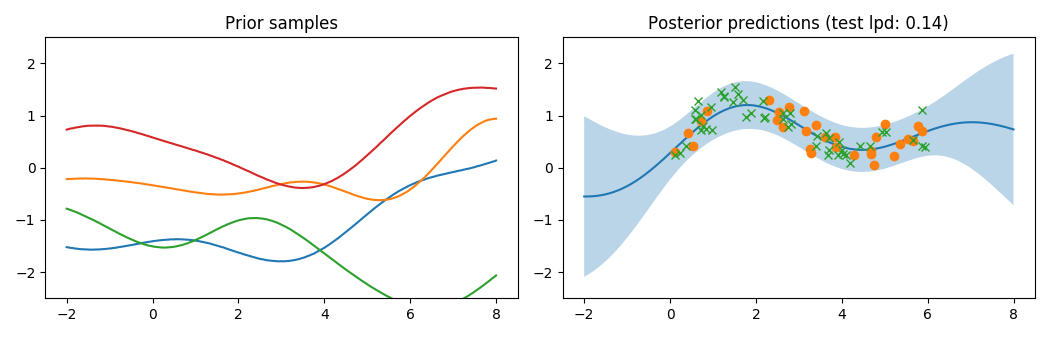
\includegraphics[height = 3.8cm]{./figures/model_selection/data2_00_model2_00.png}}
\onslide*<2>{Dataset 1: \\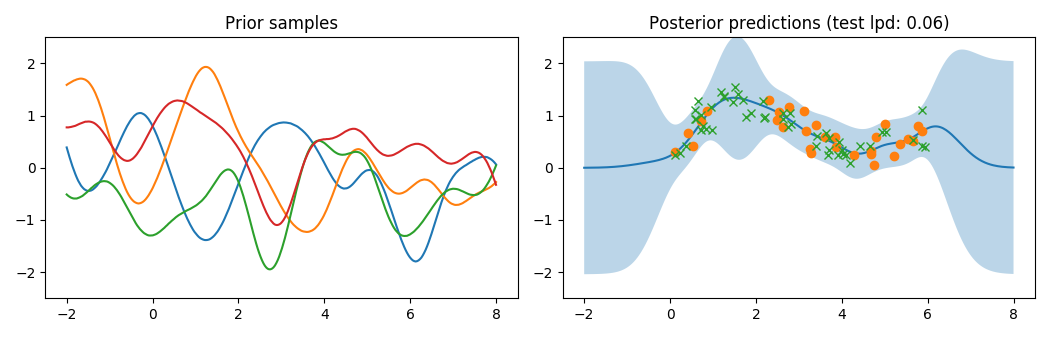
\includegraphics[height = 3.8cm]{./figures/model_selection/data2_00_model0_63.png}}
\onslide*<3>{Dataset 1: \\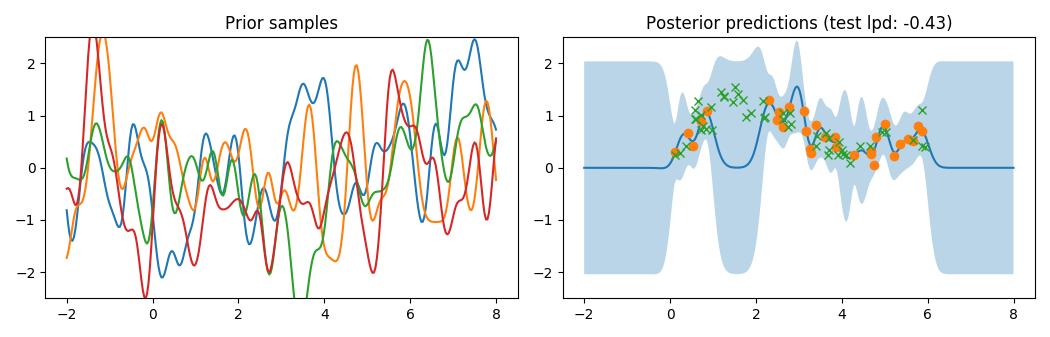
\includegraphics[height = 3.8cm]{./figures/model_selection/data2_00_model0_20.png}}
\onslide*<4>{Dataset 2: \\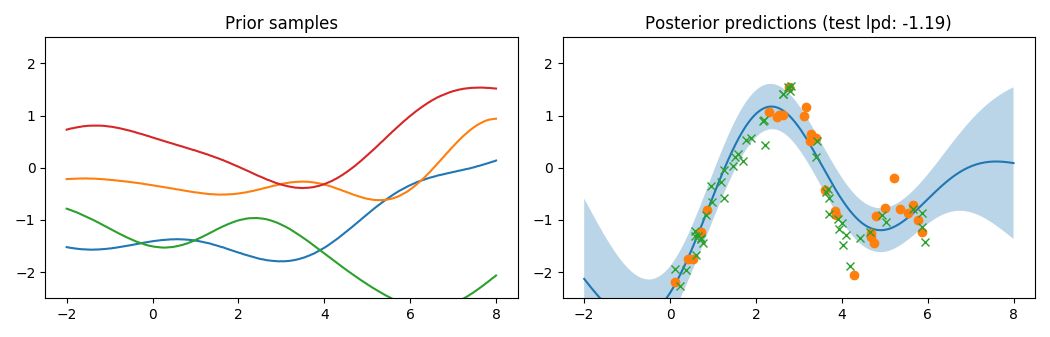
\includegraphics[height = 3.8cm]{./figures/model_selection/data0_63_model2_00.png}}
\onslide*<5>{Dataset 2: \\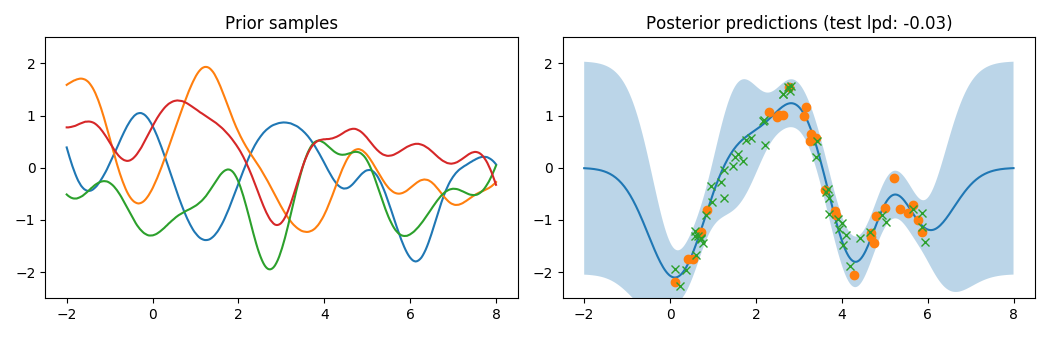
\includegraphics[height = 3.8cm]{./figures/model_selection/data0_63_model0_63.png}}
\onslide*<6>{Dataset 2: \\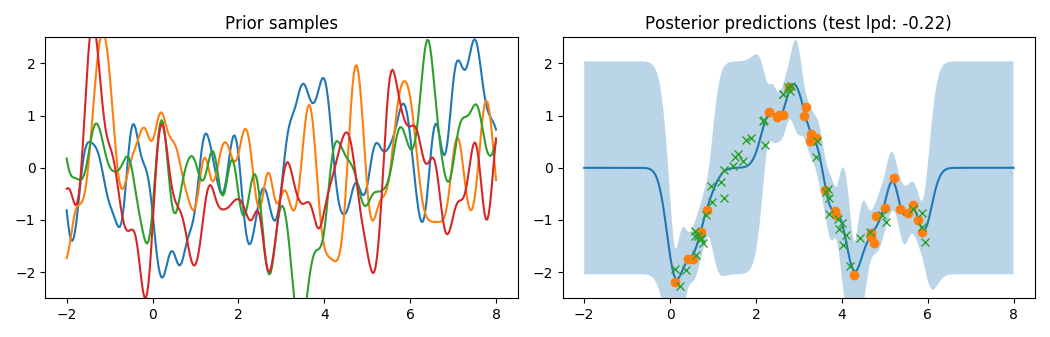
\includegraphics[height = 3.8cm]{./figures/model_selection/data0_63_model0_20.png}}
\onslide*<7>{Dataset 3: \\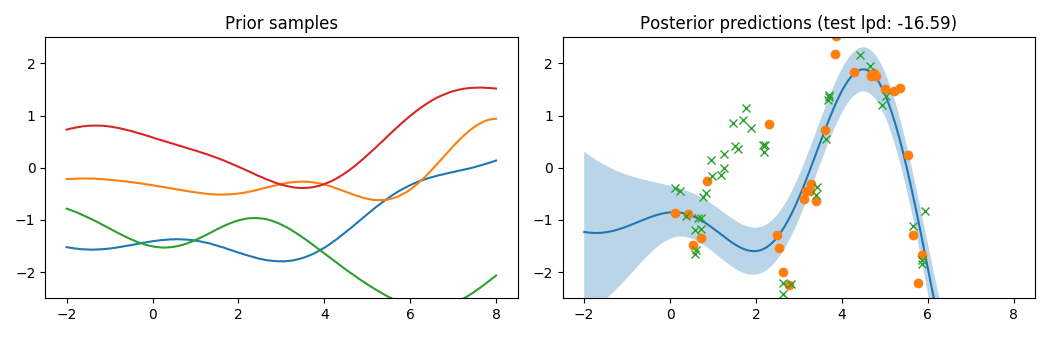
\includegraphics[height = 3.8cm]{./figures/model_selection/data0_20_model2_00.png}}
\onslide*<8>{Dataset 3: \\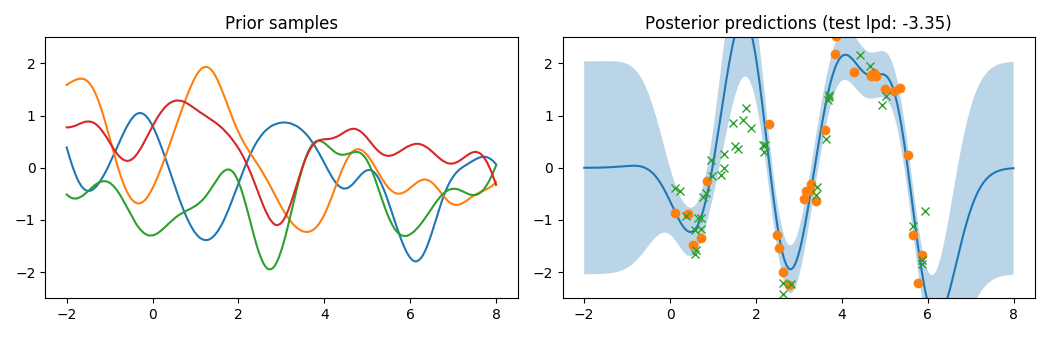
\includegraphics[height = 3.8cm]{./figures/model_selection/data0_20_model0_63.png}}
\onslide*<9>{Dataset 3: \\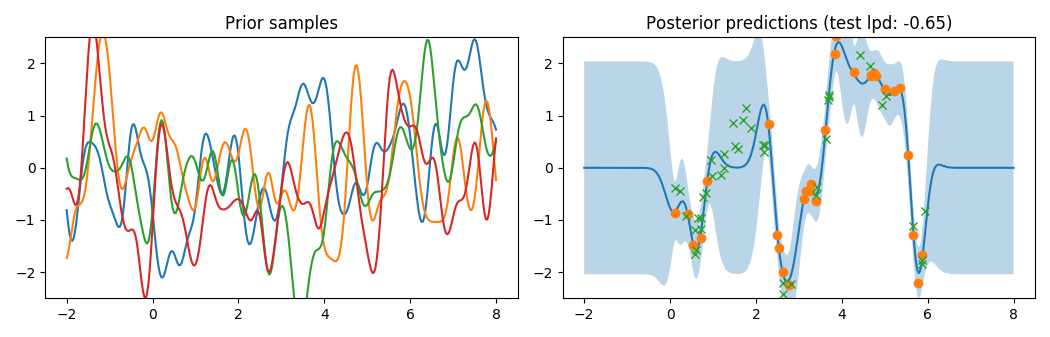
\includegraphics[height = 3.8cm]{./figures/model_selection/data0_20_model0_20.png}}
\end{figure}
% \vspace{-0.5cm}
\begin{itemize}
\item More flexibility in the model
\item Faster increase in uncertainty away from data
\end{itemize}
\end{frame}



\begin{frame}{What is model selection}
\begin{itemize}
\item Given a prior, we can make predictions with uncertainty.
\item Different priors make different predictions of different quality.
\item Different tasks need different priors.
\end{itemize}

\pause

\begin{center}
\Large How do we select the right prior for the task? \\
\vspace{0.5cm}
\pause
$\to$ Model selection
\end{center}

\end{frame}


\begin{frame}{Bayesian approach}
Let's follow the Bayesian approach.

\begin{center}
Hyperparameters are simply  \pause \\
yet another {\Large \bf unobserved quantity} \\\pause
which we can infer with {\Large \bf Bayes' rule}. \pause
\end{center}

\begin{align}
p(\gpfdp|\vy, \theta) = \frac{p(\vy, \gpfdp | \theta)}{p(\vy|\theta)} = \frac{p(\vy|\gpfd, \theta)p(\gpfdp|\theta)}{p(\vy|\theta)}
\end{align}

\begin{itemize}
\item I use $\gpfdp$ as shorthand for $\begin{bmatrix}f(\mat X)\transpose & f(\vx_*)\end{bmatrix}\transpose \in \Reals^{N+1}$.
\item Here, I drop the conditioning on the inputs.
\item If \textit{explicitly asked} on an exam, you must be able to correctly specify what inputs a distribution depends on.
\end{itemize}
\end{frame}


\begin{frame}{Bayes for hyperparameters}
  Bayes' rule for everything:
  \begin{align}
    p(\gpfdp, \theta \given \vy) = \frac{p(\vy, \gpfdp, \theta)}{p(\vy)} = \frac{p(\vy\given \gpfd, \theta) p(\gpfdp|\theta) p(\theta)}{p(\vy)}
  \end{align}
  \pause
\vspace{-0.5cm}
  \begin{align}
    \qquad\quad\, = \underbrace{\frac{p(\vy\given \gpfd, \theta) p(\gpfdp|\theta)}{p(\vy\given \theta)}}_{p(\gpfdp|\vtheta,\vy)} \underbrace{\frac{p(\vy\given \theta) p(\theta)}{p(\vy)}}_{p(\theta\given \vy)}
  \end{align}
  \pause

  Posterior over $f$ and $\theta$ consists of two parts \pause
  \begin{enumerate}
  \item The original posterior over $f$, \pause
  \item A posterior over $\theta$ using the \emph{marginal likelihood}:
    \begin{align}
      p(\vy | X, \theta) = \int p(\vy | f(X), X, \theta) p(f(X)|\theta) \calcd{f(X)}
    \end{align}
  \end{enumerate}
\end{frame}

\begin{frame}{Marginal likelihood surface}
  \begin{enumerate}
  \item To predict $f$, we need to take into account all uncertainty over both $f$ and $\theta$
    \begin{align}
      p(f(\vx^*)|\vy, X) = \int p(f(\vx^*)\given \vy, X, \theta) p(\theta\given \vy, X) \calcd{\theta}
    \end{align}

  \item We take a $p(\theta)$ which is uniform over a large range of values
    \begin{align}
      p(\theta|\vy, X) \approx \frac{1}{Z}p(\vy\given X, \theta)
    \end{align}
  \end{enumerate}
\end{frame}

\begin{frame}{Marginal likelihood surface}
Visualisation of hyperparameter posterior $p(\theta | \vy, X) \approx p(\vy | X, \theta)$:
\vspace{-0.6cm}
\begin{figure}[T]
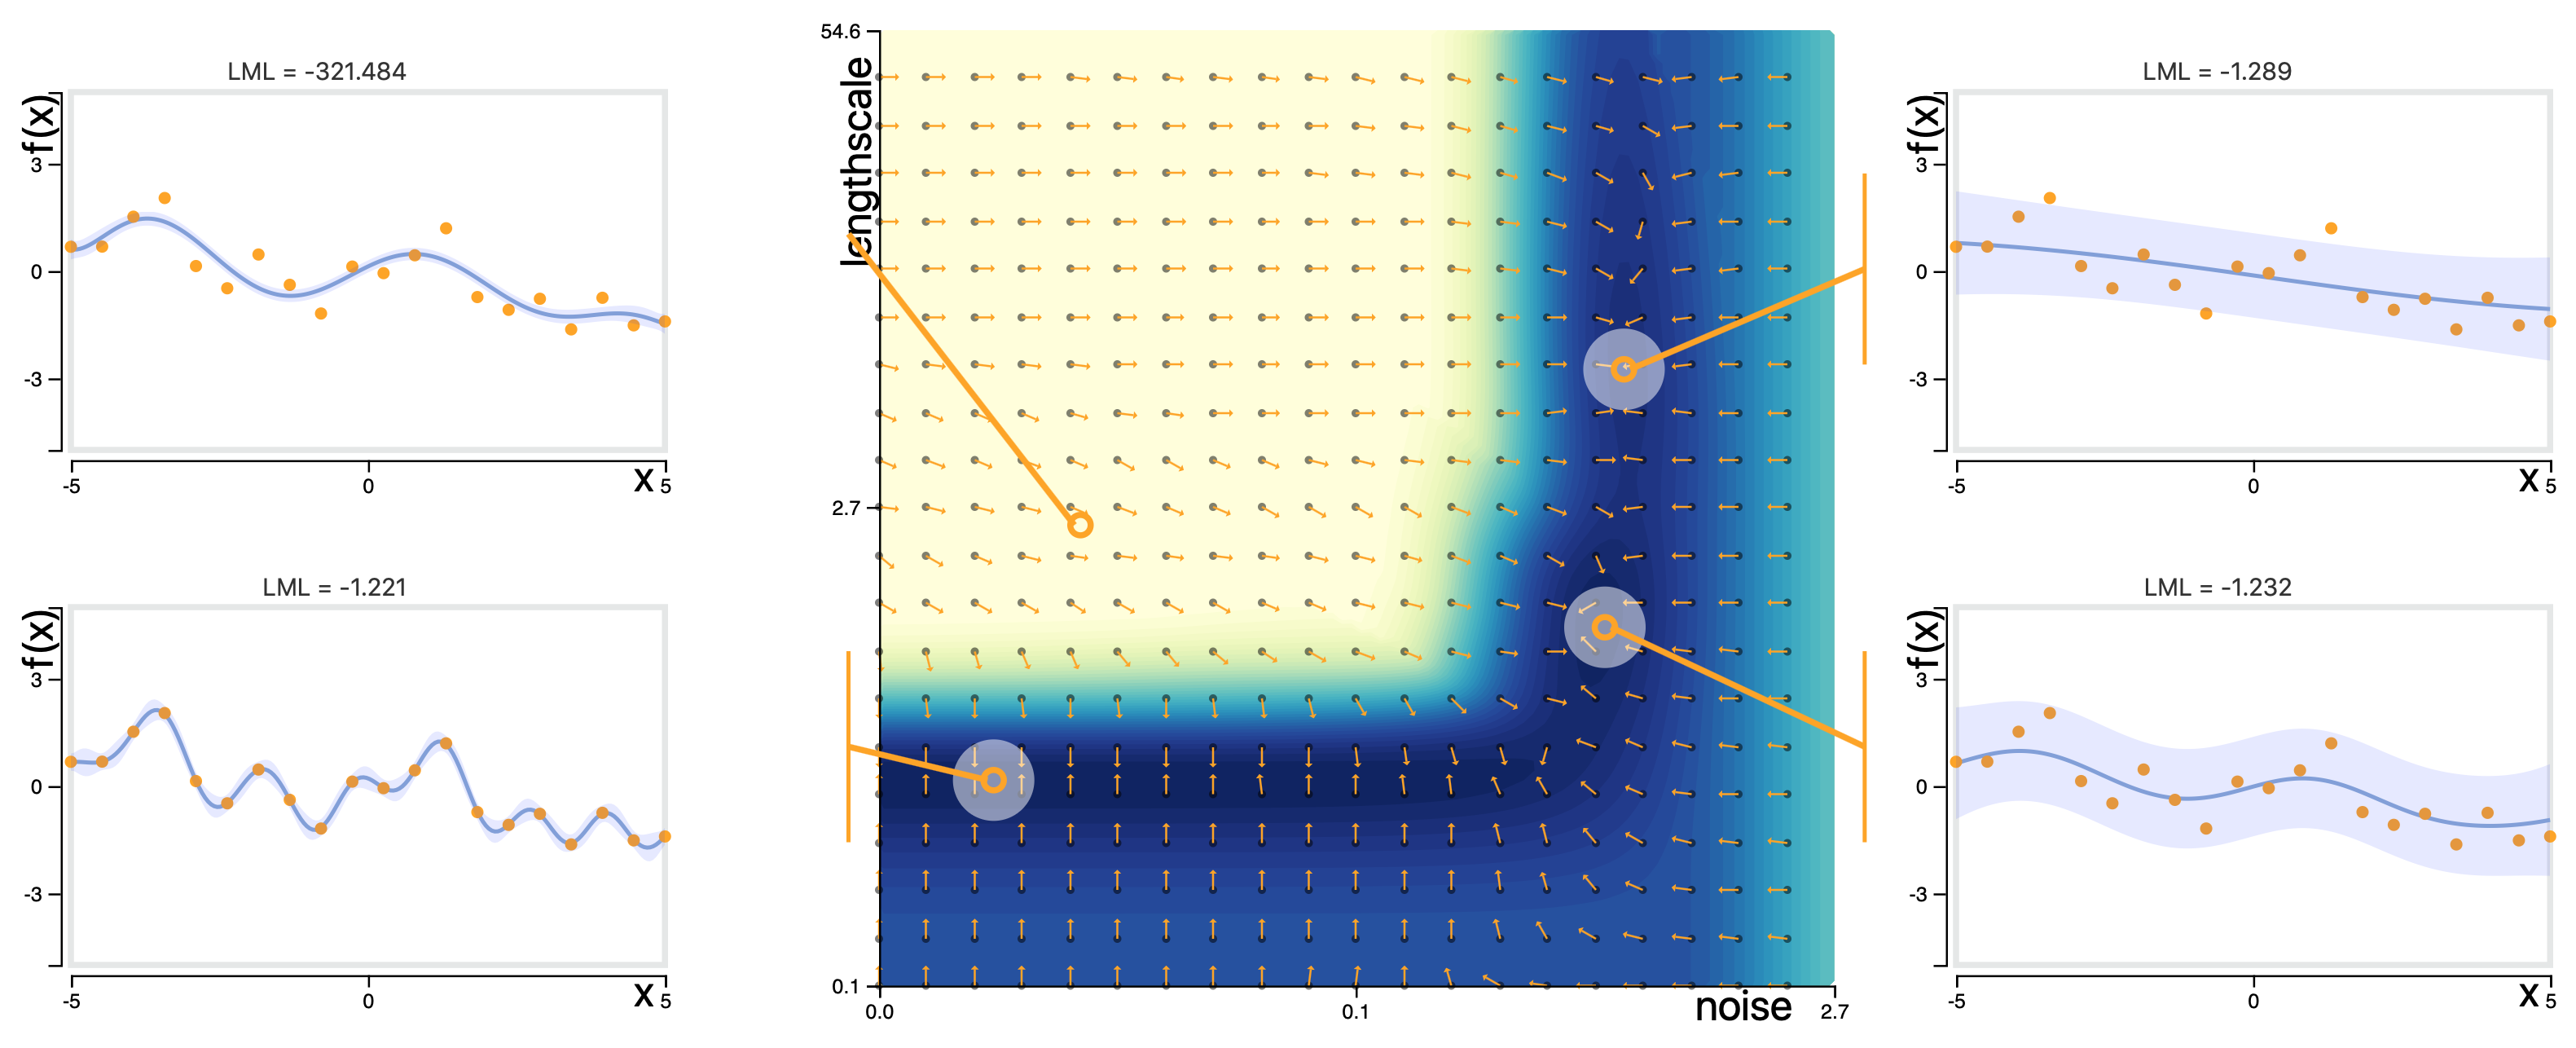
\includegraphics[height = 5.0cm]{./figures/model_selection/marglik-surface.png}
\end{figure}
\vspace{-0.3cm}
\begin{itemize}
  \item Several plausable hyperparameters
  \item Predictions should take posterior uncertainty into account!
\end{itemize}
\begin{center}
  Try for yourself: \url{https://drafts.distill.pub/gp/}
\end{center}
\end{frame}

\begin{frame}{Intractable inference}
To make a prediction, we need to compute
    \begin{align}
      p(f(\vx^*)|\vy, X) = \int p(f(\vx^*)\given \vy, X, \theta) p(\theta\given \vy, X) \calcd{\theta}
    \end{align}
\pause
No closed-form solution for this integral. Inference is \textbf{intractable} \pause :(
\pause
\begin{align}
p(\theta\given \vy, X) = \frac{p(\vy\given X, \theta) p(\theta)}{{\color{red}p(\vy|X)}} = \frac{p(\vy\given X, \theta) p(\theta)}{{\color{red}\int p(\vy|\theta, X)p(\theta) \calcd{\theta}}}
\end{align}
\pause
\begin{itemize}
  \item We can compute the \emph{relative} plausibility of a finite number of hyperparameters,
  \item but the prediction needs to know the weight relative to the total volume of \emph{all} hyperparameters.
\end{itemize}
\end{frame}


\begin{frame}{Practical solution}
\begin{itemize}
  \item Many approximations exist when closed-form solutions don't (variational, MCMC, ...) \pause
  \item One pragmatic approximation is to \emph{ignore uncertainty in $\theta$}.
\end{itemize}
\pause
\begin{align}
p(\theta|\vy, X) \approx \delta(\theta - \hat{\theta}) \,, \qquad \hat{\theta} = \argmax_\theta p(\vy\given\theta, X) p(\theta)
\end{align}
\begin{itemize}
\item Maximum a-posteriori (MAP) approximation \pause
\item Found by numerically optimising $p(\vy|\theta, X)p(\theta)$, using \emph{gradients}
\end{itemize}
\end{frame}


\begin{frame}{Numerical optimisation}
\begin{figure}[T]
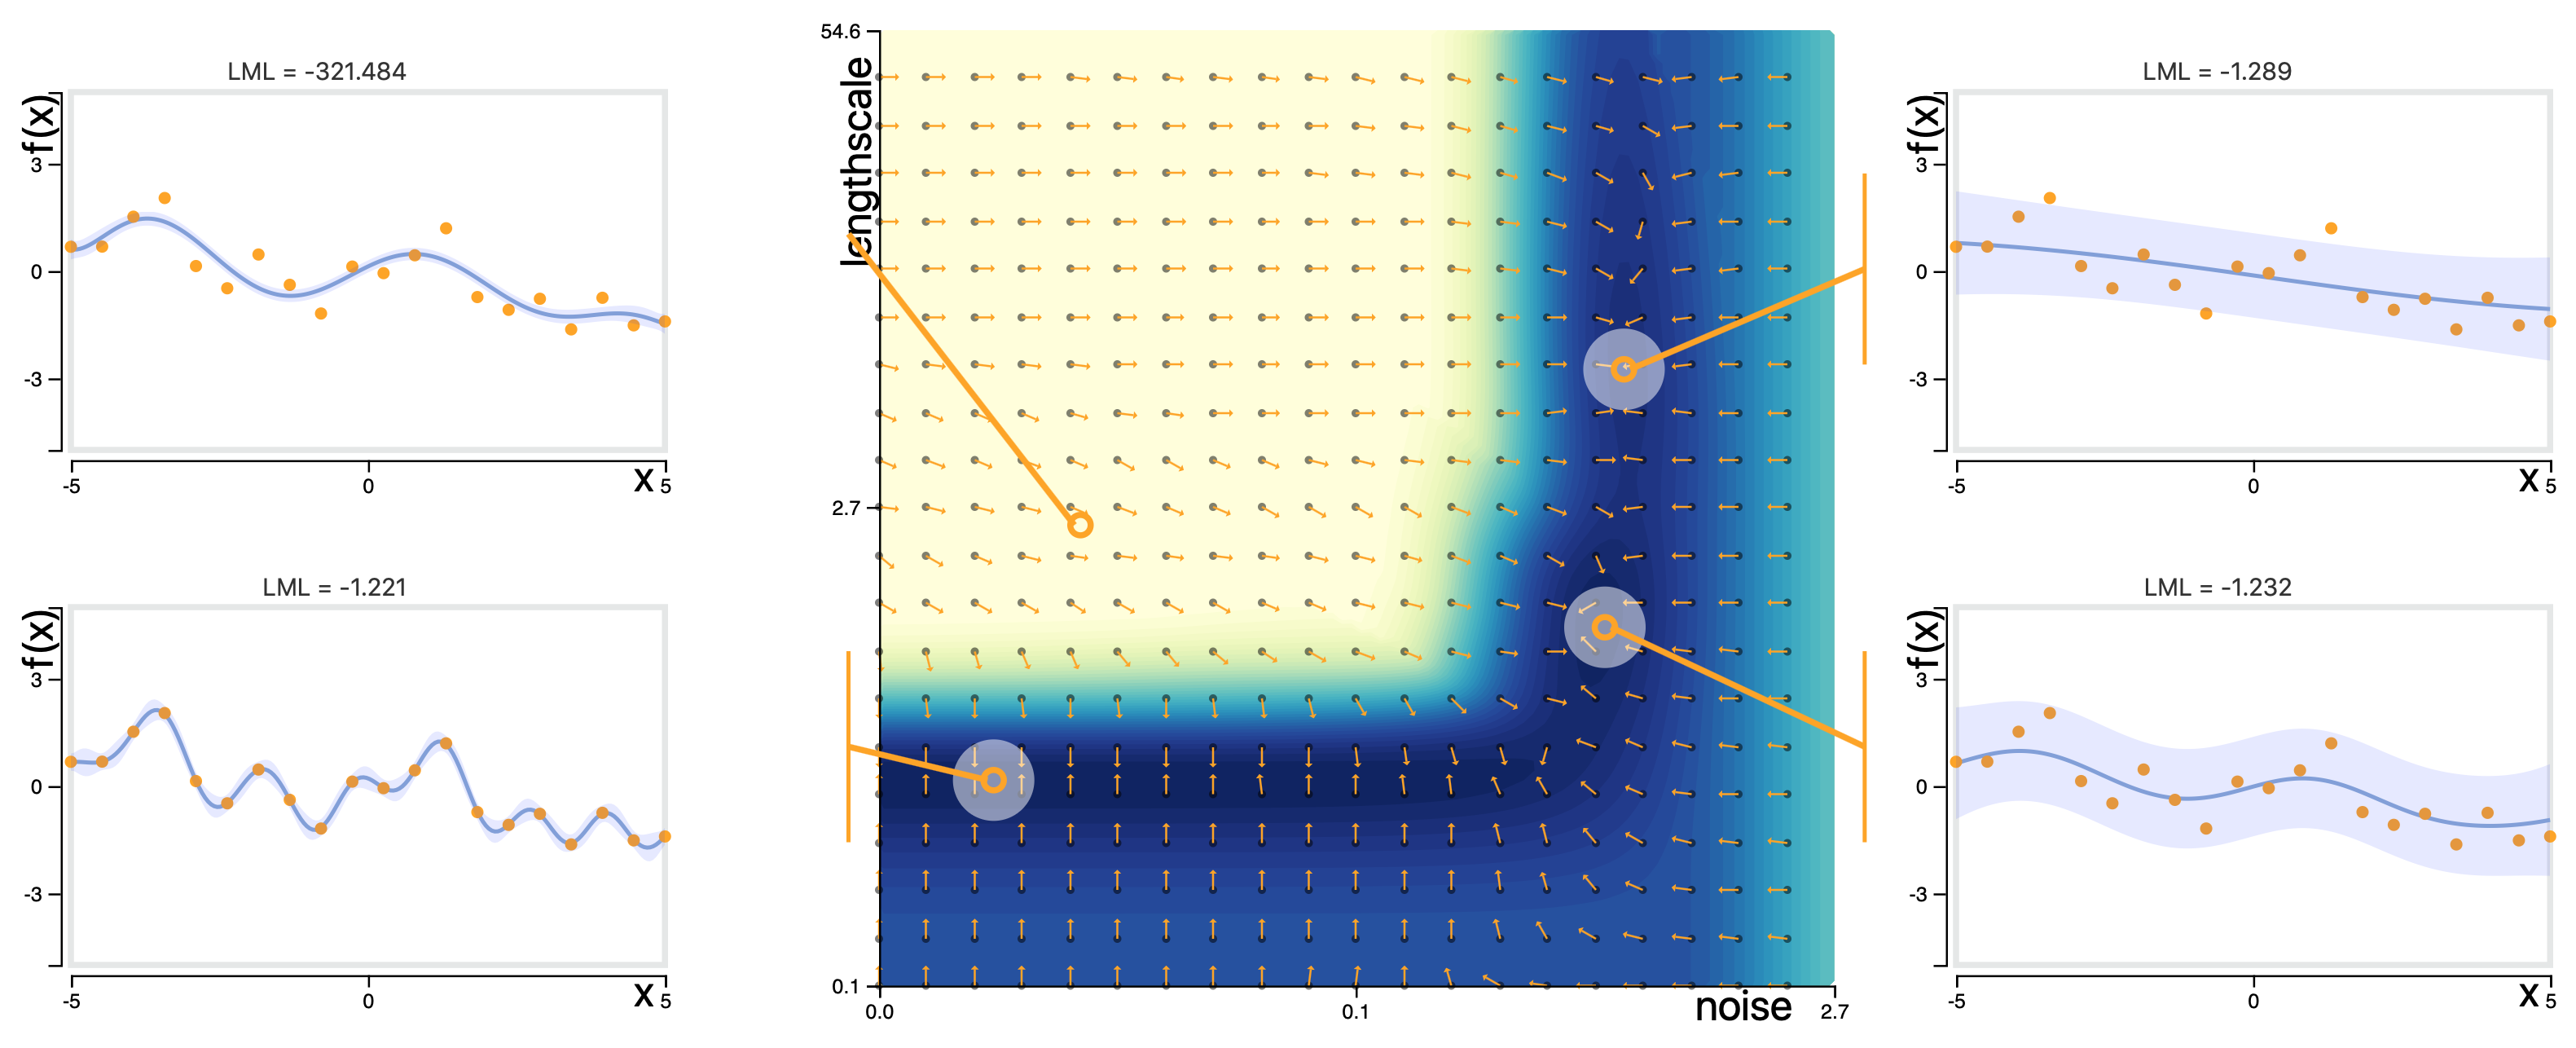
\includegraphics[height = 5.0cm]{./figures/model_selection/marglik-surface.png}
\end{figure}

\begin{itemize}
\item Gradients indicated on image push you towards optima
\item Surface is non-convex, so we can end up in multiple solutions
\item Which one we end up in, depends on starting point
\end{itemize}
\end{frame}



\begin{frame}{How to optimise}
We are searching for $\argmax_\theta p(\vy\given\theta, X) p(\theta)$, so
\begin{itemize}
  \item Random re-starts at different locations
  \item Pick the $\theta$ with the highest value of $p(\vy\given\theta, X) p(\theta)$
  \item Pick a good initialisation based on your data
\end{itemize}
\pause
\vspace{-0.3cm}
\begin{figure}
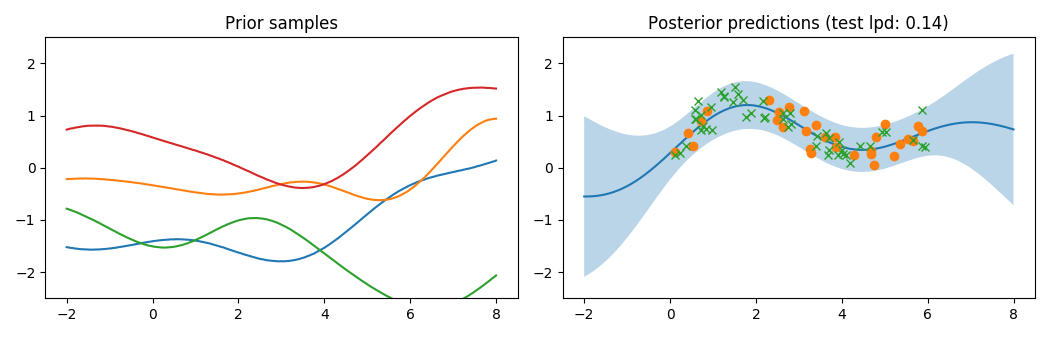
\includegraphics[height = 3cm]{./figures/model_selection/data2_00_model2_00.png}
\end{figure}
\vspace{-0.4cm}
\begin{itemize}
\item Lengthscale appropriate to input range
\item Variance appropriate to output range
\item Noise scale based on how ``predictable'' you think the dataset is
\end{itemize}
\end{frame}


\begin{frame}{When is MAP ok?}
\begin{itemize}
  \item More data $\rightarrow$ less uncertainty in $\theta$\\
$\rightarrow$ delta more appropriate
  \item More data $\rightarrow$ fewer local optima \\
$\rightarrow$ optimisation more likely to work
\item More parameters in $\theta$, same data $\rightarrow$ uncertainty increases \\
$\rightarrow$ delta less appropriate
\end{itemize}
\end{frame}


\begin{frame}
\frametitle{Example}
\vspace{-5mm}
\onslide*<1>{
\begin{figure}
\centering
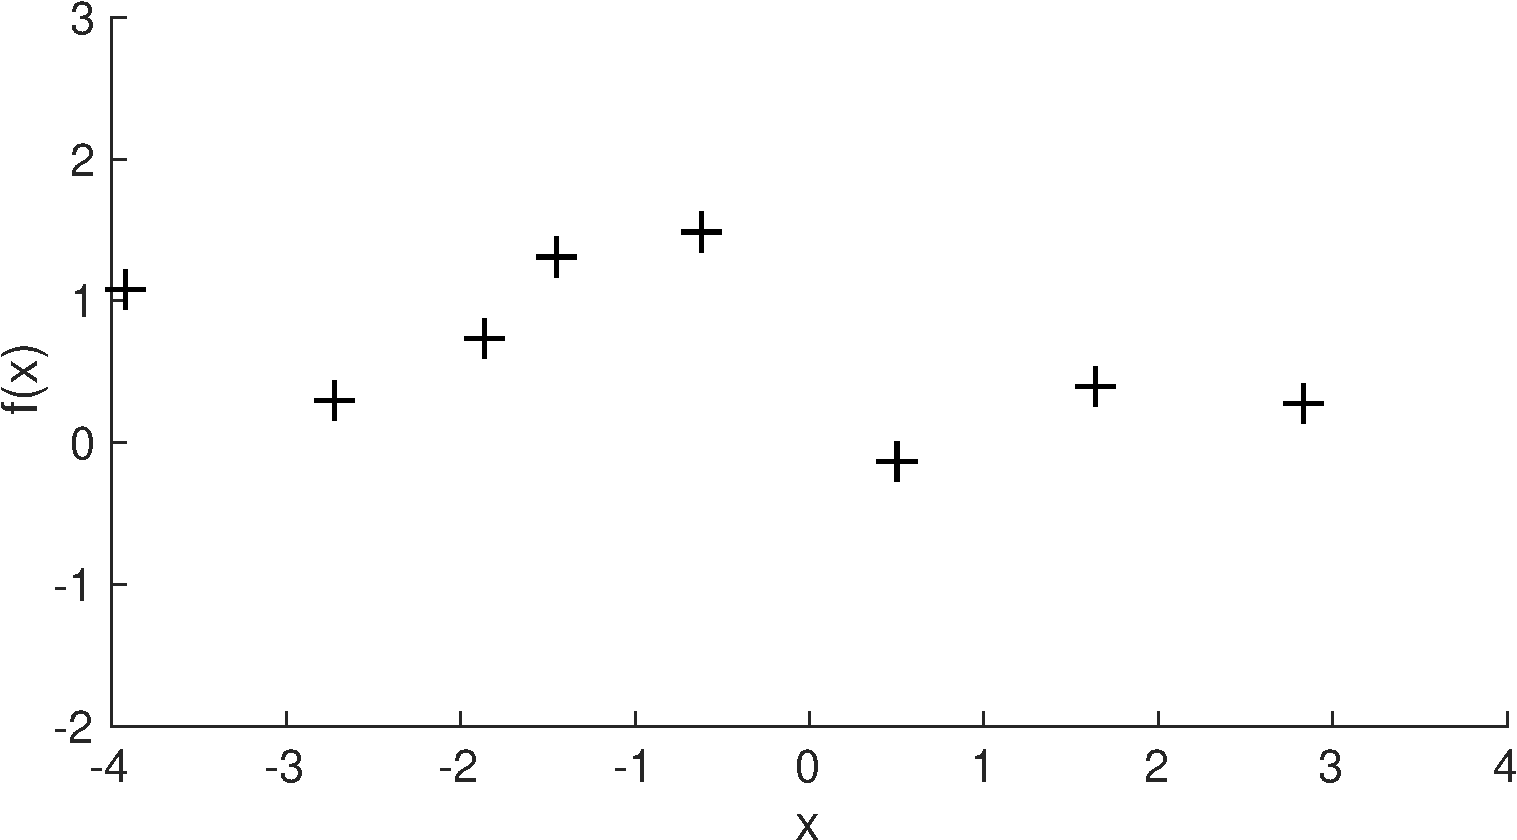
\includegraphics[height = 6cm]{./figures/model_selection/data_model_selection}
\end{figure}
}
\onslide*<2>{
\begin{figure}
\centering
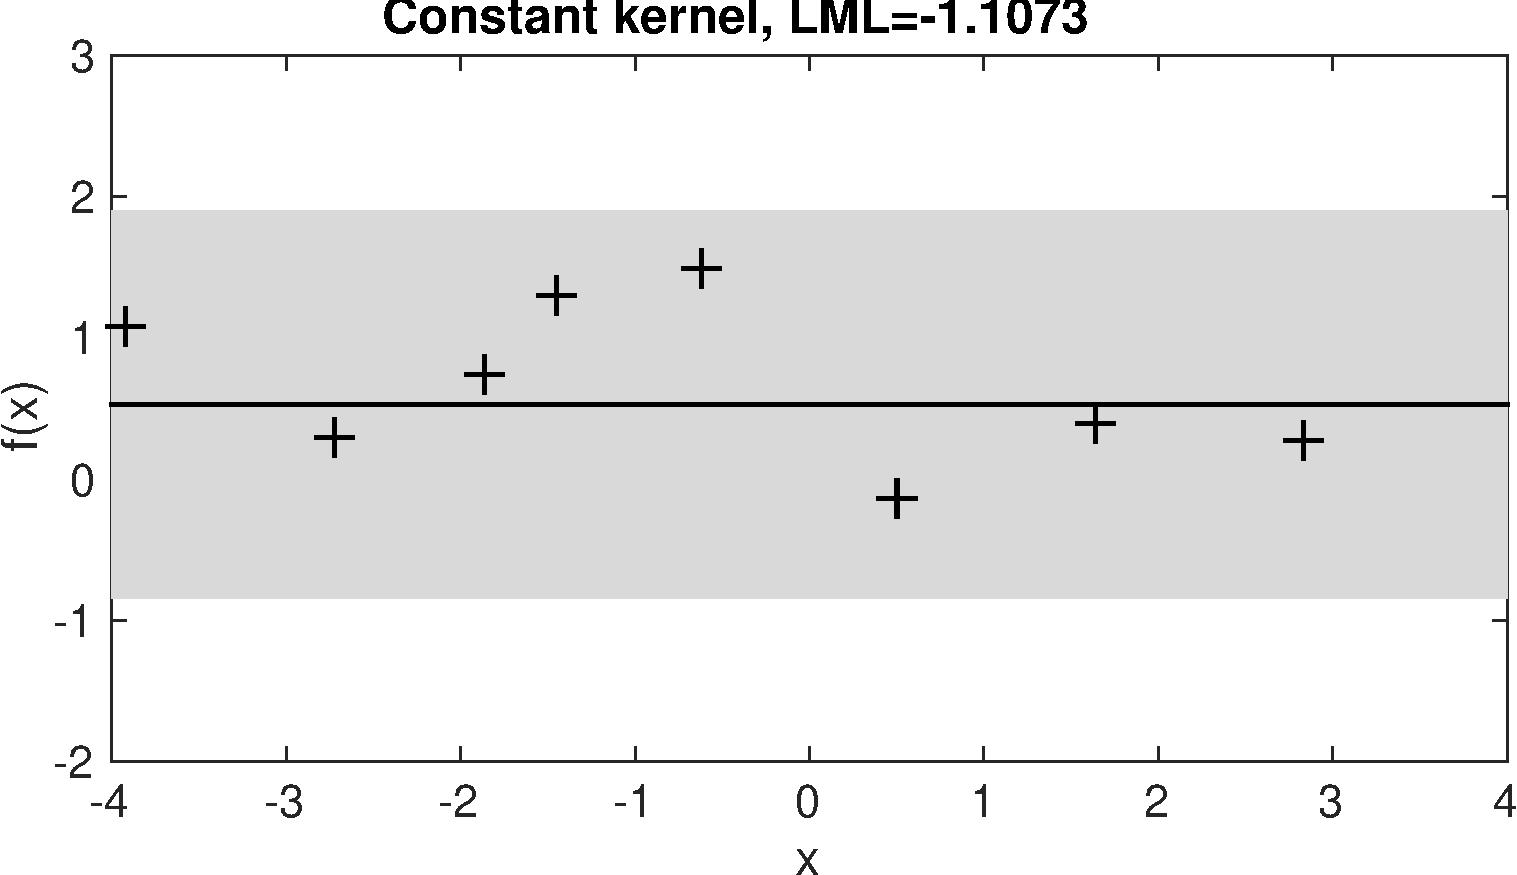
\includegraphics[height = 6cm]{./figures/model_selection/model_selection_const}
\end{figure}
}
\onslide*<3>{
\begin{figure}
\centering
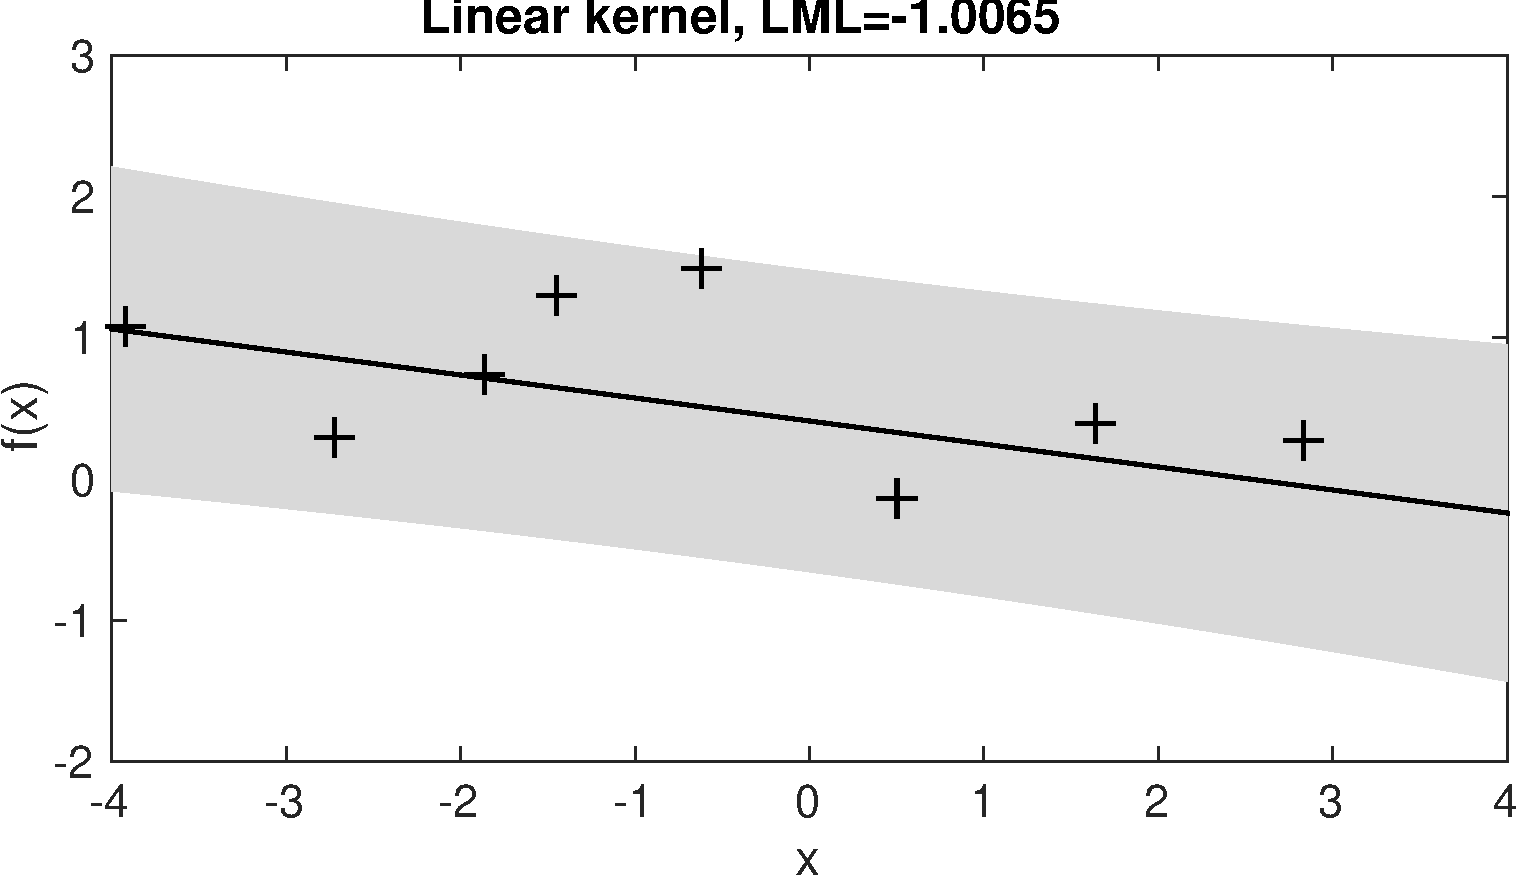
\includegraphics[height = 6cm]{./figures/model_selection/model_selection_lin}
\end{figure}
}
\onslide*<4>{
\begin{figure}
\centering
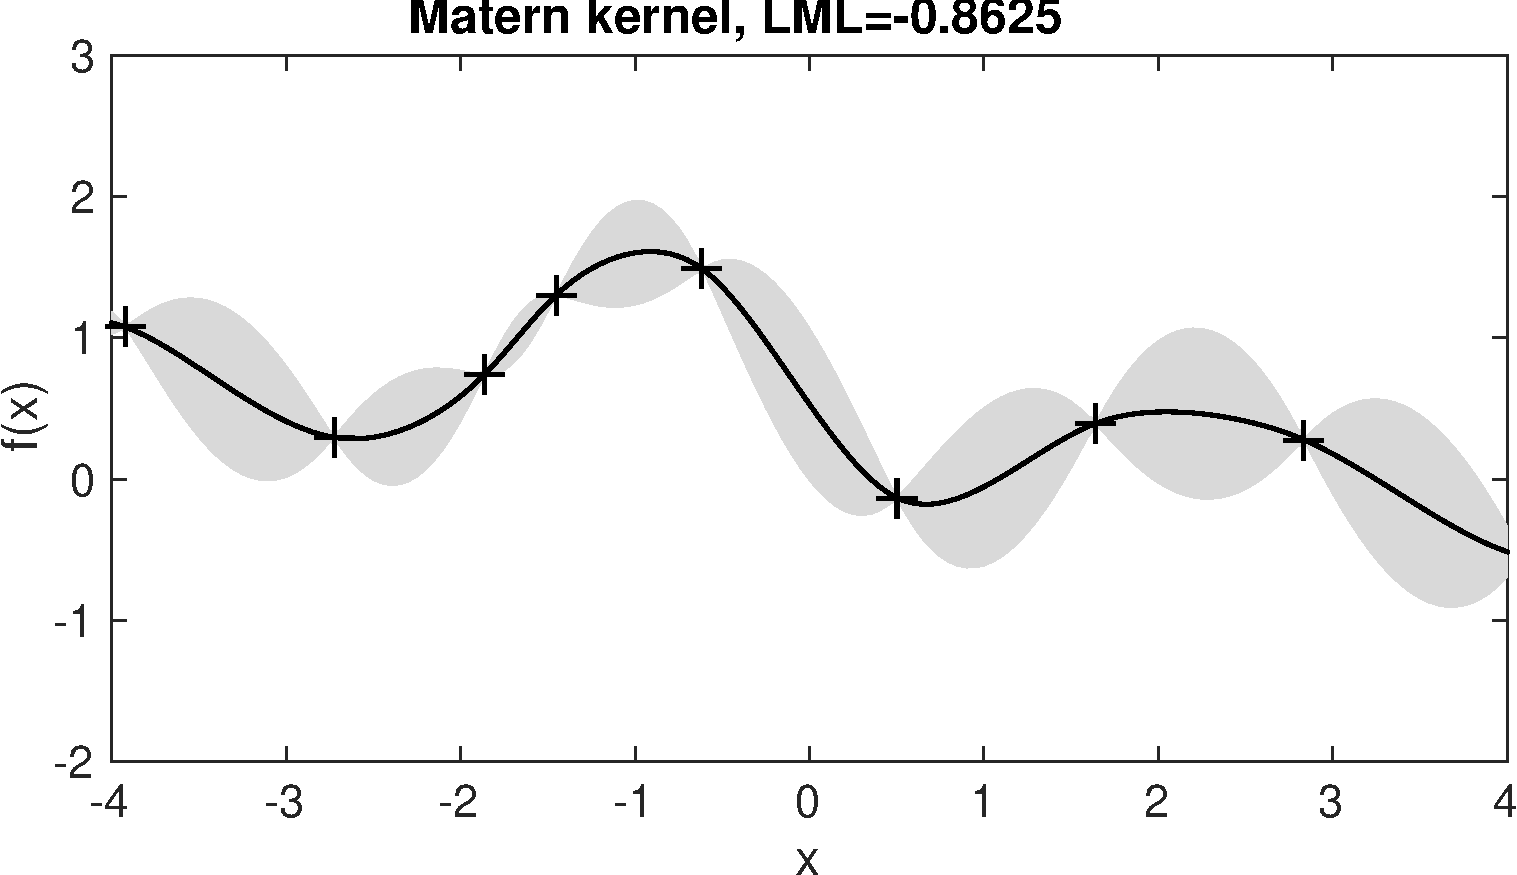
\includegraphics[height = 6cm]{./figures/model_selection/model_selection_matern3}
\end{figure}
}
\onslide*<5>{
\begin{figure}
\centering
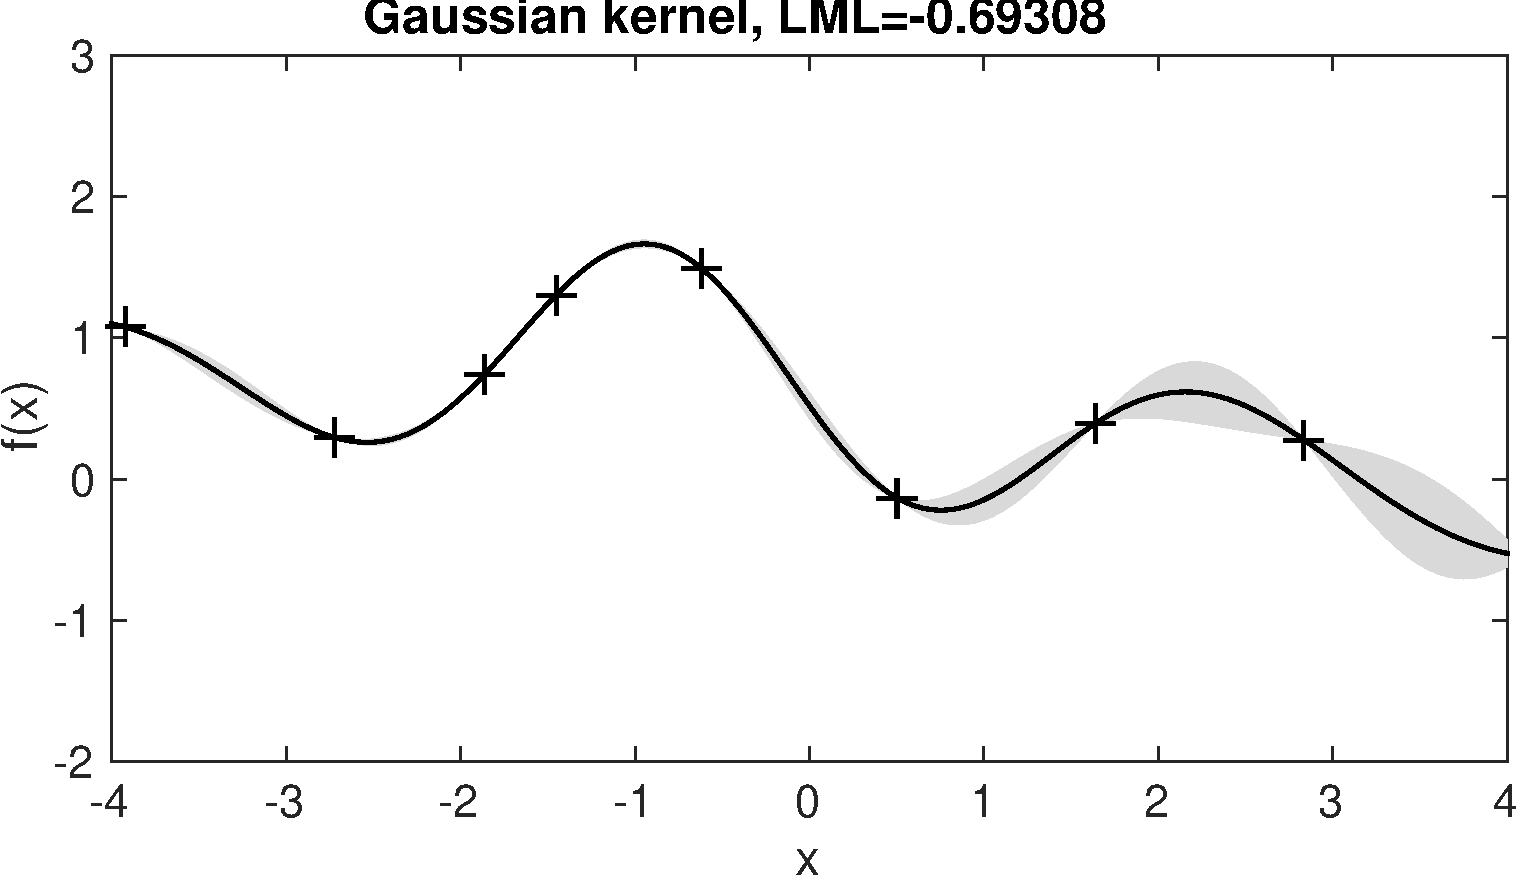
\includegraphics[height = 6cm]{./figures/model_selection/model_selection_gauss}
\end{figure}
}
\vspace{-3mm}
\begin{itemize}
\item Four different kernels (mean function fixed to $m\equiv 0$)
\item MAP hyper-parameters for each kernel
\item Log-marginal likelihood values for each (optimized) model
\end{itemize}
\end{frame}


\begin{frame}{Fitting a real dataset}
See Jupyter notebook \texttt{mauna.ipynb}.
\end{frame}



\begin{frame}{Conclusion}
\begin{itemize}
\item The assumptions in the prior distribution affect the posterior, and its generalisation characteristics
\item We can apply Bayes rule to find the posterior over hyperparameters
\item Bayesian integrals are hard, but maximising the posterior (MAP) can be reasonable
\end{itemize}
\end{frame}

\begin{frame}{Further reading}
\begin{itemize}
\item \nocite{gpml} Rasmussen \& Williams. \textit{Gaussian Processes for Machine Learning}, chapter 5.
\end{itemize}
\end{frame}








% \nocite{Roberts2013, Krause2008, Deisenroth2015b, Deisenroth2009,Deisenroth2015, Calandra2014,Calandra2015a,
%   Calandra2014b,  Deisenroth2011c,
%   Quinonero-Candela2003a, Rasmussen2006, Sutton1998, Bertsekas2005,
%    Jones1998, Brochu2009, Osborne2009, Bertone2016, Baroukh2014,
%   Deisenroth2012d, Deisenroth2012,Frigola2013,Kocijan2004,Quinonero-Candela2005}


%%%%%%%%%%%%%%%%%%%%%%%%%%%%%%%%%%%%%%%%%
% REFERENCES
%%%%%%%%%%%%%%%%%%%%%%%%%%%%%%%%%%%%%%%%%
\begin{frame}[t,allowframebreaks]
\frametitle{References}
\linespread{1.0}
\tiny
\bibliographystyle{abbrv}
\bibliography{../includes/pi-literature.bib}
\end{frame}



\end{document}
%%% Local Variables: 
%%% mode: latex
%%% TeX-master: t
%%% End: 
